\documentclass[output=paper]{langsci/langscibook}
\ChapterDOI{10.5281/zenodo.3972866}
\author{Chenchen Song\affiliation{University of Cambridge}}
\title{Categorizing verb-internal modifiers}

% \chapterDOI{} %will be filled in at production

\abstract{In this chapter, I propose a novel theory to explain the syntactic
    and semantic characteristics of a class of previously lesser studied verb
    modifiers, namely the non-heads of compound verbs like \emph{double-check}
    and \emph{hand-wash}. Such verb-internal modifiers are more widely used in
    \ili{English} contrary to common impression, and they are also a very productive
    \isi{compounding} strategy in East Asian languages like Chinese and \ili{Japanese}.
    However, in the familiar European languages they are either systematically
    missing (e.g.\ in \ili{Romance} languages) or subject to odd movement constraints
    (e.g.\ in \ili{German}), even when these languages do not equally lack compound
    nouns. The theory I propose makes use of a defective categorizer that bears
    a lexically unvalued categorial feature. It agrees with the categorial
    feature on the base verb and results in a word-internal \isi{adjunction}
    structure. The model is solely based on Simplest \isi{Merge} without resorting to
Pair \isi{Merge} or Root \isi{incorporation}, can be readily extended to the nominal
domain, and nicely relates the typology of verb-internal modifiers to the
parametrization of \isi{verb movement}\is{verb movement|seealso{head movement}}.}

\maketitle

\begin{document}\glsresetall

\section{Introduction}\label{sec1}

There is a long line of syntactic research on \glsunset{VM}\glsdesc{VM}s
(\glspl{VM}, \posscitealt{Kiss2002} term), most fruitfully on verbal particles,
as represented by those in \ili{Germanic} languages (e.g.\ \ili{German}
\textit{\textbf{ein}-kaufen}\footnote{The hyphen is used for expository
convenience and does not indicate orthography.} `in-buy; to shop', cf.
\citealt{DeheEtal2002}, \citealt{Haiden2006}, and references therein) and
Hungarian (e.g.\ \textit{\textbf{ki}-mos} `out-wash; to wash out', cf.
\citealt{Kiss1987}, \citeyear{Kiss2002}, \citeyear{Kiss2008},
\citealt{Hegedus2013}). A standard view on the particle-like \glspl{VM} is that they
are base-generated as V-complements, e.g.\ in small clauses
(\citealt{Taraldsen1983}, \citealt{Kayne1985} et seq.). They are
modifiers in the broad sense that non-heads in a phrase enrich the head's
meaning.

There is still another type of \gls{VM} which has received comparatively less
attention in traditional generative studies. Observe the examples in
\REF{ex:mod}.

\ea\label{ex:mod}
    \textit{double}-check, \textit{second}-guess, \textit{proof}-read,
    \textit{dry}-clean, \textit{hand}-wash, \textit{stir}-fry,
    \textit{sleep}-walk, \textit{window}-shop, \textit{baby}-sit,
    \textit{breast}-feed, \textit{hitch}-hike \dots
\z

\noindent While the italicized components in \REF{ex:mod} are intuitively also
modifiers, these complex verbs are traditionally treated as compounds, i.e.
lexical items, whose internal structures are a matter of morphology rather than
syntax. In other words, the \glspl{VM} in \REF{ex:mod} are word-internal; call them
\glspl{VIM}. Unlike verbal particles, \glspl{VIM}\is{verb-internal modifiers} are neither V-complements nor
secondary predicates. Rather, they modify the base verbs in the same way
adverbs modify VPs.

Contrary to the common impression that compound verbs are unproductive in
English, \ili{English} speakers are evidently no less capable of creating items like
\REF{ex:mod}\footnote{Syntacticians are contributing quite a bit to this list.
    A quick Google search finds the following examples in the published
literature: {\it set/pair/self-merge}, {\it head/phrasal/A/\={A}/wh-move}, {\it
left/right-adjoin}, etc.\ All are attested in the \Prs.\Tsg{} form, so they are
unequivocally used as verbs.} than e.g.\ speakers of Chinese, which is
considered very productive in compound verbs.\footnote{The productivity of
    compound verbs is influenced by multiple factors, e.g.\ \REF{ex:mod}-type
    compounds in Chinese are extremely productive because they form standard
prosodic words \citep{Feng1997}.} If \isi{compounding} is part of our language
competence, it should be subject to general linguistic principles and,
crucially, only rely on computational mechanisms made available by \gls{UG}, hence no
compounding-specific rule. \glsunset{DM}\glsdesc{DM} (\gls{DM},
\citealt{HalleMarantz1993} et seq.) treats syntax (essentially \isi{Merge},
\citealt{HauChoFit2002}) as the only generative engine in the human language
faculty (single engine hypothesis, \citealt{Marantz2001b}). I take this as my
point of departure.

With these theoretical advances, many issues about \isi{compounding} need to be
carefully rethought, as witnessed by the numerous works within \gls{DM} (i.a.\
\citealt{Zhang2007,Harley2009,Hu2013,NishiyamaOgawa2014,Bauke2016,deBeldervanKoppen2016,Song2017COPiL}).
This chapter furthers this exploration by putting forward a new perspective on
the structure of \glspl{VIM}\is{verb-internal modifiers}. To be specific, I categorize \glspl{VIM}\is{verb-internal modifiers} via a
lexically unvalued ``defective categorizer'' and assign them the categorial value
of the base verbs via \isi{Agree}.  This new model has three major advantages. First,
it is solely based on Simplest \isi{Merge} and labeling\is{labelling} \citep{Chomsky2013}, making
no use of Pair \isi{Merge} or Root \isi{incorporation}. Second, it can be extended to the
nominal domain, unifying verbal and nominal \isi{compounding}. Third, it
relates the typological availability of \glspl{VIM}\is{verb-internal modifiers} to the parametrization of
\isi{verb movement}.

This chapter is organized as follows. In \Cref{sec2}, I illustrate the
categorial properties of \glspl{VIM}\is{verb-internal modifiers} with cross-linguistic data, concluding that they
are simultaneously lexical and functional and qualify as word-internal
adjuncts. In \Cref{sec3}, I review two minimalist approaches to \isi{adjunction},
arguing that the labeling-based model is more favorable. In \Cref{sec4}, I
propose and motivate such a model, featuring a defective categorizer and a
Root-joining schema. In \Cref{sec5}, I further discuss the theoretical and
typological predictions of the model. \Cref{sec6} concludes.

\section{The categorial status of verb-internal modifiers}\label{sec2}

As a general observation, \glspl{VIM}\is{verb-internal modifiers} can be of any lexical category\is{lexical
    categories}, as in \REF{ex:lexcat}.\footnote{Chinese and \ili{Japanese}
    have no P-origin \glspl{VIM}\is{verb-internal modifiers} because they lack the English-type P items
    (cf.\ \citealt{HuangEtal2009,Tsujimura2013,Song2017}). I leave P-related
    issues aside due to space limit.}

\ea\label{ex:lexcat}
\ea \ili{English}\\ \textit{hand}\textsubscript{N}-wash,
\textit{stir}\textsubscript{V}-fry, \textit{dry}\textsubscript{A}-clean,
\textit{under}\textsubscript{P}-score
\ex Chinese\\ \textit{sh\v{o}u}\textsubscript{N}-x\v{\i}e `hand-write; to
handwrite', \textit{zǒu}\tss{V}-dú \enquote*{walk-read; attend a day school},
\textit{d\`{a}}\textsubscript{A}-xi\`{a}o `big-laugh; to laugh loudly'
\ex \ili{Japanese}\\ \textit{se}\textsubscript{N}-ou `back-carry; to carry on back',
\textit{oshi}\textsubscript{V}-taosu `push-topple; to push down (topple by
pushing)', \textit{chika}\textsubscript{A}-zuku `close-attach; to get near'
\z
\z

\noindent %\glspl{VIM} can be N, V, and A in all the three genealogically unrelated languages. \ili{English} also has P-origin ones. However, due to various complications concerning the P category, e.g.\ its non-purely lexical nature (cf.\ \citealt{Svenonius2008}, \citeyear{Svenonius2010}), event structure relevance (e.g.\ \textit{he has} *(\textit{\textbf{out}})-\textit{grown his brother}), and cross-linguistic heterogeneity (cf.\ \citealt{HuangEtal2009}, \citealt{Tsujimura2013}, \citealt{Song2017}), a thorough untangling of P-origin \glspl{VM} would take us too far afield. Therefore, I largely leave them aside in my discussion and merely make the prediction that if a P-origin \gls{VM} is generated in the same way as the N/V/A-origin ones in \REF{ex:lexcat}, i.e.\ as an \gls{VIM}\is{verb-internal modifiers}, it should behave in the same way as well.

One may be tempted to conclude that \glspl{VIM}\is{verb-internal modifiers} simply belong to their separate
lexical categories. This conclusion is problematic in several ways. First, it
misses the generalization that \glspl{VIM}\is{verb-internal modifiers}, whatever their lexical source, all perform
the same function (i.e.\ modification). This issue does not arise in traditional
studies where \glspl{VIM}\is{verb-internal modifiers} have no syntactic relevance whatsoever, but in the
single-engine approach, we need to syntactically formalize this
``beyond-lexical'' equivalence class.

Second, even the lexical labels themselves may not be tenable, for \glspl{VIM}
and the respective \isi{lexical categories} do not have much in common beyond the
superficial resemblance. Consider the ``N'' modifiers in \REF{ex:lexcat}. They
repel typical nominal distributions such as pluralization and quantification in
English \REF{ex:n-eng}, classification in Chinese \REF{ex:n-chi}, and adjective
modification in all the three languages \REF{ex:n-all}.

\ea\label{ex:n}
\ea[*]{hands-wash, {*} one hand-wash}\label{ex:n-eng}
\ex[*]{y\`{\i} zh\={\i} sh\v{o}u-xi\v{e} `one \Clf{} hand-write'}\label{ex:n-chi}
\ex[*]{pretty hand-wash, {*} qi\v{a}o sh\v{o}u-xi\v{e} `skillful hand-write',
    {*} aoi se-ou `blue back-carry'}\label{ex:n-all}
\z
\z

\noindent Since no distributional criterion can tell us \textit{hand},
\textit{sh\v{o}u}, and \textit{se} are nouns, the label N can only come from
the impression that they are usually used as nouns elsewhere (the same is true
for the other \gls{VIM}\is{verb-internal modifiers} labels). However, such impression-based categorization
is unreliable, because the same form may be reused in different categories,
e.g.\ \textit{a \textbf{hand}}\textsubscript{N} vs.\ \textit{to
\textbf{hand}}\textsubscript{V} \textit{in the essay}. The invariant part here
is the Root $\sqrt{\textrm{\textsc{hand}}}$ rather than its categorized
products.

%The impression that \textit{hand} is usually used as a noun may simply be due to the higher frequency of (and familiarity with) the nominal concept (i.e.\ the body part).

Third, some \glspl{VIM}\is{verb-internal modifiers} do not fall in any existing lexical category\is{lexical
categories}, such as the prefixes in \textit{\textbf{re}-build},
\textit{\textbf{un}-fold}, \textit{\textbf{dis}-close},
\textit{\textbf{mis}-understand}, etc.\ They perform the same ``adverbial''
function as the other \glspl{VIM}\is{verb-internal modifiers} we have seen but cannot be categorized by
impression. Similarly, in some \ili{Japanese} V-V compounds, the first
component is so bleached\footnote{The bleaching is not only semantic but also
phonological, e.g.\ \textit{tott}<\textit{tori}, \textit{hin}<\textit{hiki},
\textit{butt}<\textit{buchi}.} that its assumed category V becomes vague, as in
\REF{ex:jap-pre}.

\ea\label{ex:jap-pre}
\textit{sashi}-semaru {`put-come.close; be imminent'}, \textit{tori/tott}-tsuku {`take-attach; cling to, be obsessed'}, \textit{hin}-mageru {`pull-bend; bend, distort'}, \textit{butt}-taosu {`hit-topple; violently topple'}\dots
\z

\noindent According to \citet{Kageyama1993}, these italicized forms have become
intensifying prefixes. Like \ili{English} \textit{re-}, \textit{un-}, etc., they
cannot be classified into any category.

%, but need to be properly labeled nevertheless.\footnote{A presupposition here is that the \glspl{VIM}\is{verb-internal modifiers}, being open-class items, are derived via at least one branching node just like content words, e.g.\ \textit{hand}\textsubscript{[\emph{n} \textsc{hand}]}, so labeling\is{labelling} is necessary (see note \ref{fn:label}).}

In sum, if we want to identify a unified syntactic category\is{syntactic
categories} for \glspl{VIM}\is{verb-internal modifiers}, the ordinary
\isi{lexical categories} are not a good place to look; the more plausible place
is their functionality instead. That is, albeit counterintuitive, \glspl{VIM}
may form a functional category. This said, however, they are not inflectional,
because canonical inflectional categories are closed classes, often with
dedicated exponents, e.g.\ \textit{-ed} for past tense. Being an open class
with no fixed exponents, \glspl{VIM}\is{verb-internal modifiers} are again more
like lexical categories.

This categorial status is reminiscent of the functionally ``recycled'' lexical
items in Biberauer (\citeyear{Biberauer2016b}, \citeyear{Biberauer2017}).
According to Biberauer, recycling effects such as \isi{grammaticalization} and
multifunctionality are a distinctive property of natural languages, reflecting
the domain-general third factor maximize minimal means. I illustrate this point
with Chinese light verbs \REF{ex:light} and classifiers \REF{ex:cl} (see
Biberauer's works for more cross-linguistic examples).

\ea \label{ex:light}
\ea
\textit{d\v{a}}-r\'{e}n {`hit-person; to hit someone' vs.}  \textit{d\v{a}}-y\'{u} {`\textsc{do}-fish; to fish'}
\ex
\textit{b\v{a}}-zh\`{u} f\'{u}sh\v{o}u {`hold-still handrail; to firmly hold
the handrail' vs.} \textit{b\v{a}}-sh\={u} d\v{a}-k\={a}i {`\Disp{}-book hit-be.open; to open the book'}
\z
\ex \label{ex:cl}
    \ea b\v{\i}j\`{\i}-\textit{b\v{e}n} {`note-book' vs.} y\`{\i} \textit{b\v{e}n} sh\={u} {`one \Clf{} book; a book'}
    \ex shu\v{\i}-\textit{b\={e}i} {`water-glass' vs.} y\`{\i} \textit{b\={e}i} shu\v{\i} {`one \Clf{} water; a glass of water'}
    \z
\z

\noindent Light verbs and classifiers have lexical origins, and they still keep
much idiosyncrasy as function words, as evidenced by the numerous same-function
items in \REF{ex:same} which are nonetheless non-interchangeable.

\ea\label{ex:same}
    \ea `Do' light verbs: \textit{d\v{a}} `hit',
        \textit{zu\`{o}} `make', \textit{n\`{o}ng} `play around' \dots{}
    \ex Disposal light verbs: \textit{b\v{a}} `hold', \textit{ji\={a}ng} `lead,
        support', \textit{gu\v{a}n} `manage' \dots{}
    \ex Classifiers: \textit{b\v{e}n} `for books',
        \textit{b\={e}i} `for liquid in glass', \textit{t\'{o}u}
        `for animals' \dots{}
    \z
\z

\noindent Similar flexibility exists in other languages, e.g.\ there are at
least four productive light verbs in \ili{English}: \textit{do}, \textit{take},
\textit{make}, and \textit{have}. The cross-linguistic widespreadness of
semi-functional items implies some basic generative strategy.
\citet[5]{Biberauer2016} identifies this strategy as adjoining featurally
underspecified elements (effectively Roots) to null functional
heads.\footnote{\label{fn5}This idea deviates from \gls{DM}. First, it relies on a
conception of Root broader than that in \gls{DM} (but closer to that in
\citealt{Borer2013}), for not only lexical but also functional forms can be
recycled (e.g.\ \textit{that}\textsubscript{D/C}). Second, it violates the \gls{DM}
assumption that Roots cannot appear without being categorized by one of the
category defining heads (the categorization assumption,
\citealt{EmbickMarantz2008}; see \citealt{Song2017roots} for a less restrictive
version compatible with Biberauer's idea).}
%
%However, given the ongoing debate regarding the exact nature of Roots and
%categorizers (cf.\ Borer \citeyear{Borer2005}, \citeyear{Borer2013}, Ramchand
%\citeyear{Ramchand2008}, \citeyear{Ramchand2017}), I leave the theoretical
%conflicts aside. \posscitet{Borer2013} definition of Root and
%\posscitet{Song2017roots} adapted Root licensing condition are potential
%bridges between Biberauer's idea and \gls{DM}.}
%
Following this idea, the functional heads\is{functional items} behind light verbs and classifiers
are Larsonian VP-shells (e.g.\ Voice, Appl, cf.\ \citealt{Lohndal2014}) and Cl
(\citealt{Borer2005,Feng2015,Huang2015}). By comparison,
the head H behind \glspl{VIM}\is{verb-internal modifiers} is much less clear-cut. It cannot simply be \gls{VIM}\is{verb-internal modifiers},
for that would entail an ad hoc formal feature (FF) [VIM] which makes little
sense in our feature system.\footnote{\label{fn6}According to
\citet{Zeijlstra2008} and Biberauer (\citeyear{Biberauer2016},
\citeyear{Biberauer2017}), FFs piggyback on substantive features, so [Person]
and [Gender] are legitimate FFs while [Affix] and [Complement] are not.} Nor
can it be any VP-shell category, because on the one hand, \glspl{VIM}\is{verb-internal modifiers} are
inside the complex verbs rather than above VP; on the other hand, while
VP-shells and Cl only recycle from V and N sources respectively (in line with
\posscitealt[36]{RobertsRoussou2003} observation that \isi{grammaticalization} is
always upwards in a functional hierarchy), H can recycle from any contentful
morpheme without categorial restriction, which makes the process more like
\emph{lexicalization}, with H systematically converting various concepts into
lexical items, just like categorizers. This effectively bears out the \gls{DM} view
that the non-heads of primary compounds are bare Roots
\citep[cf.][]{deBelder2017}, though I deviate from (almost all) previous \gls{DM}
approaches to \isi{compounding} from RootP \isi{incorporation} (e.g.\ \citealt{Harley2009})
to Root--Root merger (e.g.\ \citealt{Zhang2007,Bauke2016}), for
reasons to be spelled out in \Cref{sec4}.

In fact, since the \gls{VIM}\is{verb-internal modifiers} is merged as a
non-complement non-projecting sister of V, it is essentially a V-adjunct, which
means H, if existent, systematically creates head \isi{adjunction}. As such, a proper
syntactic model of \glspl{VIM}\is{verb-internal modifiers} relies on an adequate theory of \isi{adjunction}. I
briefly review theories of \isi{adjunction} in the next section.

\section{Minimalist approaches to adjunction}\label{sec3}
\subsection{Pair Merge}\label{sec3.1}

One may wonder: if \glspl{VIM}\is{verb-internal modifiers} are adjuncts, why do we need to give them any
functional head at all? Shouldn't their modifier role be self-evident? These
questions implicitly take \isi{adjunction} and its asymmetric effect for granted,
which is undesirable given the (beyond-)explanatory goal of the minimalist
program.

The standard minimalist approach to \isi{adjunction} is Pair \isi{Merge} (Chomsky
\citeyear{Chomsky2000}, \citeyear{Chomsky2004}), which takes two syntactic
objects α,  β and yields an ordered pair \tuple{α, β}. α (the adjunct) is
attached to β from a separate plane, which is invisible to and thus cannot
interfere with the primary-plane derivation. Following this idea, \isi{adjunction}
does not need any functional head\is{functional items} but is a special operation. However, Pair
Merge sacrifices the minimalist and evolutionary advantages of the theory,
because, as \citet[52]{Collins2017} points out, it has to be stipulated as an
independent \gls{UG}\is{Universal Grammar} operation, which goes against the \glsunset{SMT}\glsdesc{SMT}
(\gls{SMT}, ``language keeps to the simplest recursive operation'',
\citealt[71]{BerwickChomsky2016}).  \citet[40]{Chomsky2013} also criticizes the
``extension of Merge'', arguing that there is no remerge, \isi{multidominance} or
late \isi{Merge} (among others), but only simple \isi{Merge}.

Also note that the motivation of Pair \isi{Merge} is empirical (``it is an empirical
fact that there is also an asymmetric operation of adjunction'',
\citealt[117]{Chomsky2004}), but its problem is conceptual. As such, if we
could give the ``empirical fact'' an alternative explanation, Pair \isi{Merge} would
no longer be needed. I will discuss such alternatives in \Cref{sec3.2}. For
now, let's turn to another problem of Pair \isi{Merge}, raised in \citet{Rubin2003}:

\blockquote[{\citealt[663]{Rubin2003}}]{We need to avoid circularity here, so
    we cannot simply say that we want adjuncts to be adjuncts, so we invoke
    pair-Merge, which creates adjuncts.  Before any two expressions are merged,
    relational terms such as \emph{adjunct}, \emph{complement}, and
\emph{specifier} are premature.}\largerpage

\noindent The problem is essentially how syntax can determine Pair \isi{Merge} is
appropriate for adjuncts. Rubin's solution is a dedicated functional head\is{functional items} Mod,
which ``forms an extended projection around all base adjuncts'' such that
``[a]ny phrase headed by Mod is subject to pair-Merge'' (p.~664). This idea is
not so different from our functional head\is{functional items} H in \Cref{sec2} and also compatible
with the \isi{Borer--Chomsky conjecture} (\glsunset{BCC}\gls{BCC},
\citealt{Baker2008}), which highlights the fundamental role of features.
However, the solution is not optimal. First, as \citet[2]{ArsenijevicSio2009}
notice, when Mod connects a modifier to a noun (both are phrases in
\citealt{Rubin2003}), it selects twice -- first the modifier and then the
noun, as in \REF{ex:modi} -- but Pair \isi{Merge} only happens in the second
selection, which makes the triggering effect of Mod inconsistent.

\ea\label{ex:modi}
    \begin{tikzpicture}[baseline=(root.base)]
        \Tree   [.\node(root){N};
                    [.{{\makebox[0pt][r]{(selector) }}Mod}
                        modifier
                        {Mod \makebox[0pt][l]{(selector)}}
                    ]
                    N
                ]
    \end{tikzpicture}
\z

Second and more relevant to us, Mod has no substantive featural basis. Though
\citet[666]{Rubin2003} specifies its semantic type as
\tuple{\tuple{e,t},\tuple{\tuple{e,t},\tuple{e,t}}} (``a function from
predicates to properties of predicates''), this only describes the function we
want Mod to perform but does not relate it to any conceptual interpretation. So
\posscitet{Chomsky1995} criticism of Agr (that it is present only for
theory-internal reasons) also applies to Mod. The above two problems may not be
unsurmountable, but they do show that Rubin's intuition can be further
developed.

%So the conclusion is, \glspl{VM} do perform a single and well-defined syntactic function, namely head modification, but in the standard minimalist theory there is no encoding for this function in categorial/featural terms. In fact, the modification relation cannot be featurally encoded in general, but must rely on some special type of combination (adjunction in traditional terms and Pair \isi{Merge} after \citealt{Chomsky1995}). In \Cref{sec3} I will further discuss the various problems surrounding this merely combinatorial approach to modification.

\subsection{Labeling}\label{sec3.2}

While \citet{Rubin2003} ``determines'' Pair \isi{Merge} and justifies its role in
\isi{adjunction}, \citet{Hornstein2009} and \citet{Oseki2015} dispense with it and
derive \isi{adjunction} via Simplest \isi{Merge} (Hornstein's ``concatenate'') plus
labeling. %\footnote{\citet{Stockwell2016} makes a similar proposal based on a non-Chomskyan labeling\is{labelling} method.}
%
Following \citet{EpsteinEtal2012}, \citet{Oseki2015} assumes when two phrases
XP and YP merge but share no feature, the merger cannot be labeled. Adopting
the label accessibility condition (LAC, \citealt[90]{Hornstein2009},
\citealt[254]{EpsteinEtal2012}),\footnote{\citet[262]{EpsteinEtal2012} deduce
    LAC from minimal search and conceive it as a third factor consequence in
    the sense of \citet{Chomsky2005}.} which states that unlabeled syntactic
    objects cannot be accessed by \isi{Merge},\footnote{This view is not unanimous,
        e.g.\ for \citet{Chomsky2013} labels are only needed by the interfaces.
    As such, the indispensability of LAC in \possciteauthor{EpsteinEtal2012}
model may turn out to be a disadvantage.} Oseki further claims that at this
stage the derivation can only proceed by letting one of XP and YP participate
in further \isi{Merge}, thus yielding the ``two-peaked'' structure in \REF{ex:peak}.
In \citeauthor{Hornstein2009}'s terms, YP ``dangles off'' the
[\textsubscript{ZP} Z XP] complex.

\ea\label{ex:peak}
    \begin{tikzpicture}[baseline=(zp.base), sibling distance=1.5cm]
    \Tree   [.\node(zp){ZP};
                Z
                [.\node(XP){XP}; ]
            ]

        \node [right=1.5cm of zp] (x) {};
        \node [right=1.3cm of XP] (YP) {YP\makebox[0pt][l]{ (=Adjunct)}};

        \draw (x.south) -- (XP.north);
        \draw (x.south) -- (YP.north);

    \end{tikzpicture}
\z

\noindent \citet[261]{EpsteinEtal2012} conceive this structure as ``two
intersecting set-theoretic \glsunset{SO}\glspl{SO}''. Crucially, one peak must
be removed (via Transfer) from the narrow syntax, which then becomes
inaccessible to later derivation, rendering the island\is{islands}
effect.\footnote{\possciteauthor{EpsteinEtal2012} main focus is the Spec-TP
subject. \citeauthor{Oseki2015} extends their model to adjuncts.}

Several issues remain unclear. First, the definition of ``peak'' is vague.
Geometrically, a peak consists of two branches, but then removing a peak
amounts to removing an entire \{XP, YP\}, which means XP cannot stay in syntax
to merge again. Second, even if XP could stay, since Transfer cannot undo
Merge, the removal of YP cannot save the second merger of XP from violating No
Tampering, and since the intersected element is contained in two sets, set
intersection inevitably leads to \isi{multidominance}. Third, for
\citeauthor{EpsteinEtal2012} the removed peak is consistently the
phase-head-complement, but this causes trouble for \citeauthor{Oseki2015}, as
it wrongly predicts that adjuncts are only ever adjoined to phase\is{phases}
heads.\is{adjunction}

%Despite all the imperfections, the two-peaked model indeed eliminates Pair \isi{Merge}, and it does so while preserving the insight that adjuncts are on a separate plane. According to \citet[267]{EpsteinEtal2012}, ZP in \REF{ex:peak} neither c-commands nor dominates YP. This resembles the ``behindance'' relation in \citet{deVries2005}, where an object is merged behind another's two-dimensional plane.\footnote{\citet[4]{Chomsky2015} warns against ``the resort to multidimensionality''. However, since trees are visualizations of more abstract relations, multidimensionality is not necessarily a problem as long as it can ultimately be explained by non-metaphorical (e.g.\ mathematical) formalization.}

While the two-peaked model is far from ideal, the labeling\is{labelling} idea behind it is
indeed more advantageous than Pair \isi{Merge}:\is{SMT|see{Strong Minimalist Thesis}}
(i) it obeys the \gls{SMT}\is{Strong Minimalist Thesis} and is evolution-friendly,
(ii) it reduces the specialness of \isi{adjunction} to specific features, in line with the BCC.
Remember that \posscitet{Rubin2003} idea was also to reduce \isi{adjunction} to a
specific category, which makes it potentially compatible with a labeling-based
approach. Thus, instead of resorting to ``unlabelable'' scenarios (e.g.\ the
two-peaked model), we could also seek a solution from scenarios where labeling
can normally proceed (as in Rubin's model). I propose a new model along this
line in \Cref{sec4}.

\subsection{Interim summary}\label{sec3.3}

To recapitulate §§\ref{sec1}--\ref{sec3}, the structure of verb-internal
modifiers (V-level adjuncts) is a tricky issue in syntactic approaches to
word-formation, partly due to the elusive categorial status of \glspl{VIM}\is{verb-internal modifiers} and
partly due to the unavailability of a satisfactory theory of \isi{adjunction}. The
two problems point to the need of a categorial account of \isi{adjunction}, e.g.\ via
a mediating functional head\is{functional items} H. As such, among previous approaches to
adjunction, those based on labeling\is{labelling} (manipulating categories) are more
advantageous than those based on Pair \isi{Merge} (a specialized \gls{UG}\is{Universal Grammar} operation).
In addition, among potential labeling-based theories those featuring
``labelable'' scenarios are more coherent than those featuring ``unlabelable''
ones.

\section{Deriving verb-internal modifiers}\label{sec4}

\subsection{How \emph{not} to merge a Root}\label{sec4.1}

As mentioned in \Cref{sec2}, the relation between H and \glspl{VIM}\is{verb-internal modifiers} is similar to
that between categorizers and Roots. Note that I did not prove the necessity of
H, but only speculated that it could potentially replace \posscitet{Rubin2003} Mod.
Two points could make this speculation suspicious. First, labeling\is{labelling} (essentially
minimal search) does not need any special head to proceed. FFs on the \isi{Merge}
input alone are enough. Second, if \glspl{VIM}\is{verb-internal modifiers} are Roots, then H can be nothing but a
categorizer (\`{a} la categorization assumption, cf.\ footnote \ref{fn5}), which
leads to a dilemma, for no existing lexical category\is{lexical categories} is adequate for
\glspl{VIM}.\footnote{Similar considerations led \citet{deBeldervanKoppen2016} to
conclude that the non-heads of some \ili{Dutch} compound nouns are bare Roots without any
functional category, not even categorizers.}%\citet{deBelder2017} recognizes
% the conflict between this empirical conclusion and the categorization
% assumption in \gls{DM} (i.e.\ all Roots must be categorized,
% \citealt{EmbickMarantz2008}) and avoids it by deriving such compounds via the
% postsyntactic \gls{DM} operation fission. I will evaluate this approach alongside the
% others later but ceteris paribus the model I am to propose avoids the same
% conflict without resorting to fission.}

This dilemma is faced by all models applying ordinary categorizers to compound
non-heads (e.g.\ \citealt{Harley2009} for compound nouns), but it does not
force us to resort to uncategorized ``floating Roots'' (e.g.\
\citealt{deBeldervanKoppen2016}) or postsyntactic Root operations (e.g.\
fission, \citealt{deBelder2017}), especially if those solutions rely on
unwarranted definitional extension of Root, which is no more desirable than
extension of \isi{Merge}. Below I will defend the conservative position that Roots
are bare (FF-less), syntactically inert (no {\textsurd}P), and must be
categorized.

To begin with, the bare Root view is faithful to the original purpose of the
Root theory, i.e.\ lexical decomposition.\footnote{See \citet[11]{Ramchand2008}
and \citet[192]{Gallego2014b} for summaries of various Root views.} Lexical
decomposition targets non-primitive lexical items (LIs) and submits that any
composite LI, be it a pure FF bundle or an FF-equipped Root, has to be
assembled from smaller atoms rather than appearing as such all of a sudden.
This is evidenced in language acquisition/change, where feature bundles are
gradually formed and further alterable.\footnote{Despite the intuition that we
    use LIs as whole units, the existence of sub-LI knowledge has never been
    denied (hence the branch ``morphology'') -- it has simply been handled by a
    separate generative engine (the lexicon). In this sense, lexical
decomposition is not introducing anything new but merely aims to capture the
sub-LI knowledge in the single-engine framework.} To wit, any theory working
with bundled features has to assume some LI forming mechanism, including
\gls{DM}.\footnote{\citet[203]{Marantz1997} conceives the \gls{DM} narrow lexicon as
``generative'', as it contains ``atomic bundles of grammatical features [that
are] freely formed, subject to principles of formation''.} However, as
\citet{Collins2017} remarks, this poses a conceptual problem, because ``that
mechanism is not Merge'':

\blockquote[{\citealt[61]{Collins2017}}]{This state of affairs seems
    undesirable for two reasons. First, humans have an unlimited capacity to
    learn and to coin new lexical items, just like they have an unlimited
    capacity to form new phrases [\dots] Second, adding a new mechanism (to
form lexical items) would increase the complexity of \gls{UG}, going against
the \gls{SMT}.}

\noindent \citeauthor{Collins2017} concludes that LIs are formed by
\isi{Merge}. So, FF-equipped Roots, if any, must also be products of
\isi{Merge}, which takes bare Roots and FFs as input.  In short, the single
engine hypothesis and \gls{SMT}\is{Strong Minimalist Thesis} together force a
bare Root view.

Following this line of thought, if Roots are stored bare
presyntactically,\footnote{This does not rule out the possibility that non-bare
Roots (just like other composite LIs and even larger phrases) could be
lexicalized and stored postsyntactically (in \gls{DM} Lists 2 and 3) or
extra-syntactically (as general experience, cf.\ \citealt{Marantz2013}).} they
must be inert in narrow syntax, which only manipulates FFs. Among others, this
means Roots cannot head or project/label, hence no {\textsurd}P (in line with
i.a.\ \citealt{Acquaviva2009}, Borer \citeyear{Borer2009}, \citeyear{Borer2014},
\citealt{Chomsky2013}, \citealt{deBelder2011} et seq., \citealt{Alexiadou2014};
contra \citealt{Cuervo2014}, \citealt{Harley2014}). Moreover, since no featural
dependency could ever be established on Root nodes, nor could they be moved or
host movement,\footnote{Thus, Roots may be conceived as adjuncts (\`{a} la
\citealt{Marantz2013}).} hence there can be no Root \isi{incorporation} (contra
\citealt{Harley2009}). The only way a Root may participate in syntactic
derivation is via categorization, either exclusively by the lexical
categorizers (as in standard \gls{DM}) or by any functional category (as in
Borer \citeyear{Borer2005,Borer2013}; \citealt{Biberauer2016,Song2017roots}).
What matters here is that there can be no floating Root, i.e.\ every Root must be
the most deeply embedded element in its workspace (a conclusion compatible with
\citealt{Marantz2001b} and \citealt{Boeckx2014}). As such, the model in
(\ref{ex:noh}a) is infelicitous, for it is impossible to categorize the
\gls{VIM}\is{verb-internal modifiers} Root without letting it project
(\ref{ex:noh}b) or remerge (\ref{ex:noh}c).\footnote{Strictly speaking,
    $\sqrt{\textrm{\textsc{vim}}}$ can only be categorized via the
    \isi{multidominance} structure in (\ref{ex:noh}c), because in (\ref{ex:noh}b)
    what the upper {\em v} categorizes is {\textsurd}P rather than
    $\sqrt{\textrm{\textsc{vim}}}$.  Besides, (\ref{ex:noh}b) wrongly predicts
\glspl{VIM} can only be V-origin.}

\ea\label{ex:noh}
\begin{minipage}[t]{.5\linewidth}
    a.  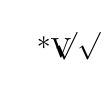
\begin{tikzpicture}[baseline=(root.base)]
        \Tree [.\node(root){*V};
                {$\sqrt{\textrm{\textsc{vim}}}$}
                [.V
                    {\em v}
                    {$\sqrt{\textrm{\textsc{verb}}}$}
                ]
            ]
        \end{tikzpicture}
\end{minipage}%
\begin{minipage}[t]{.5\linewidth}
    b. 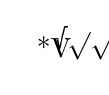
\begin{tikzpicture}[baseline=(root.base)]
        \Tree [.\node(root){*V};
                {\em v}
                [.{{\textsurd}P}
                    {$\sqrt{\textrm{\textsc{vim}}}$}
                    [.V
                        {\em v}
                        {$\sqrt{\textrm{\textsc{verb}}}$}
                    ]
                ]
            ]
        \end{tikzpicture}
\end{minipage}\\
\begin{minipage}[t]{.5\linewidth}
    c. \begin{tikzpicture}[baseline=(root.base)]
        \Tree   [.\node(root){*V};
                    \node(vim){$\sqrt{\textrm{\textsc{vim}}}$};
                    [.V
                        {\em v}
                        {$\sqrt{\textrm{\textsc{verb}}}$}
                    ]
                ]

        \node [left=.7cm of root] (X) {X};
        \node [left=.6cm of vim] (x) {\emph{x}\vphantom{$\sqrt{\textsc{vim}}$}};
        \draw (X.south) -- (x.north);
        \draw (X.south) -- (vim.north);
\end{tikzpicture}
\end{minipage}
\z

\noindent Note that (\ref{ex:noh}c) is the two-peaked structure in
\Cref{sec3.2}. Despite its infelicity, the idea that
$\sqrt{\textrm{\textsc{vim}}}$ may be categorized in \isi{adjunction} is insightful.
Therefore, if we could overcome the \isi{multidominance} problem, (\ref{ex:noh}c) may
well become a felicitous model. I will further pursue this route in
\Cref{sec4.2}. For now, let's turn to another infelicitous structure in
\REF{ex:rrm}.

\ea\label{ex:rrm}
%{\upshape
%\qtreecenterfalse
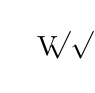
\begin{tikzpicture}[baseline=(root.base)]
    \Tree [.\node(root){V}; {\em v} [.{$\textsurd$P} {$\sqrt{\textrm{\textsc{vim}}}$} {$\sqrt{\textrm{\textsc{verb}}}$} ] ]
\end{tikzpicture}
%}
\z

\noindent This is the \isi{compounding} model adopted in i.a. \citet{Zhang2007},
\citet{Borer2013}, Bauke (\citeyear{Bauke2014,Bauke2016}) and
\citet{deBeldervanKoppen2016}. A clear problem with it is the symmetric
relation between the two Roots, which means there is no way to determine which
Root is the modifier and which is the verb at \gls{LF}, nor can they be
algorithmically linearized at PF. \citet{Borer2013} resorts to Root
incorporation to yield the asymmetry, but this operation is illegitimate under
the bare Root view, as FF-less objects cannot be moved.\footnote{De Belder
(\citeyear{deBelder2017}) proposes a fission-based variant of \REF{ex:rrm},
where the two Root nodes are ``split'' postsyntactically and the asymmetry is
yielded by ``the order of insertion''. I do not have space to evaluate this
approach, but \emph{ceteris paribus} the model I will propose later is free
from postsyntactic operations and thus potentially more parsimonious.} For more
thorough arguments against direct Root-Root merger see \citet{Song2017roots}.

With (\ref{ex:noh}--\ref{ex:rrm}) ruled out, we are left with only one structure
to derive \glspl{VIM}\is{verb-internal modifiers}, i.e.\ [H {$\sqrt{\textrm{\textsc{vim}}}$}]-[{\em v}
{$\sqrt{\textrm{\textsc{verb}}}$}], where the two Roots are separately licensed
before being joined together. The necessity of a functional head\is{functional items} H is thus
proved, not by the requirement of labeling\is{labelling} but by the nature of Root.

\subsection{Defective categorizer}\label{sec4.2}

Further examination of the structure [H {$\sqrt{\textrm{\textsc{vim}}}$}]-[{\em
v} {$\sqrt{\textrm{\textsc{verb}}}$}] reveals that H and {\em v} must share
some feature(s), for otherwise the structure is unlabelable.\footnote{Here I
follow Chomsky's (\citeyear{Chomsky2013}, \citeyear{Chomsky2015}) conception
that all branching nodes (i.e.\ all products of Merge) must be equipped with a
label at the interfaces. See \citet{Boskovic2016tlr}, \citet{BaukeRoeper2017} for
looser positions and Collins (\citeyear{Collins2002} et seq.) for a label-free
system.} However, H cannot simply be {\em v}, because that would make the
structure symmetric just like \REF{ex:rrm} and its two branches formally
undistinguishable (distinctness\is{categorial distinctness} is an important interface principle, cf.
\citealt{Richards2010}). Rather, H and {\em v} should be simultaneously
homogeneous and non-identical, and ideally the distinction should not be
achieved by bundling extra features into H/{\em v}, for that would go against
the spirit of lexical decomposition. Remember that in \Cref{sec2} H was likened
to categorizers, and that in \Cref{sec4.1} the ordinary \gls{DM} categorizers were
ruled out. As such, a simple hypothesis about H is that it is a special
categorizer.

To identify H, therefore, we need a better understanding of categorizers and
their place in the inventory of functional categories. A first point to note is
that terms like ``categorizer'', ``categorial feature'', and ``categoryless'' are
used loosely in the literature, because if items without a categorizer are
categoryless, then categoryless items would include not only Roots, but also T,
Asp, Num, etc.\ In other words, if categorial features (largely limited to [N],
[V], [A]) are what define categories (as the term literally suggests), then
various functional categories would end up being non-categories. Obviously,
these are not what \gls{DM} is expected to predict; what the above terms really
mean are ``lexical categorizer'', ``lexical categorial features'', and
``lexical-category-less'' instead. So, our mission is to identify a special {\em
lexical} category.

Despite their intuitive straightforwardness, \isi{lexical categories} are a
notoriously disputed area in minimalism. As content words are decomposed into
categorizers and Roots, the previously held \isi{lexical categories} become
functional in nature. However, ``lexical'', ``noun'', ``verb'', etc.\ do not follow
the nomenclature of functional categories (FF-based, piggybacking on
substantive features, cf.\ note \ref{fn6}) and need to be either renamed or
redefined. Two representative approaches exist in this regard.
\citet{Borer2005} denies the existence of dedicated categorizers and treats
traditional \isi{lexical categories} as distributional contrasts that are only
definable as ``categorial complement spaces'' of functional projection series,
e.g.\ D-Num-Cl is ``nominal'' while C-T-Voice is ``verbal''
(\citealt{Biberauer2016} has a similar view). On the other hand, Panagiotidis
(\citeyear{Panagiotidis2015}, \citeyear{Panagiotidis2017}) endows the
categorial features [N] and [V] with interface substantiveness, letting them
represent two ``fundamental interpretive perspectives''
(\glsunset{FIP}\glspl{FIP}) -- ``sortality'' and ``extending into
time'':

\blockquote[{\citealt[lecture 1, p.\ 4]{Panagiotidis2017}}]{Sortality will have
    to be associated with {\em individuation}, number, quantification etc.\ ---
    realised as functional categories Number, Determiner etc.\ ``Extending into
    time'' will be the seed of events and causation, and will require event
    participants, a way to encode length of event and relation between time
intervals etc.\ -- realised as an event projection / argument, Voice, Aspect,
Tense.}

The two approaches are not necessarily incompatible. Considering many
conventional labels have turned out to be mixtures of heterogeneous concepts
(e.g.\ IP/CP are extended domains,
Merge\textsubscript{MP}\,=\,Merge\textsubscript{PoP}\,+\,labeling\footnote{MP =
    {\em Minimalist Program} \citep{Chomsky1995}, PoP = {\em problems of
projection} \citep{Chomsky2013}.}), lexical categorial labels like ``noun'' and
``verb'' may also have multiple dimensions that could (and should) be
unbundled.  Specifically, we can conceive ``noun'', ``verb'', etc.\ as
distributional patterns following Borer while having an FIP-introducing
functional layer in each pattern following Panagiotidis. This layer may be
identified as the ``categorizer'' but is not really the original \gls{DM}
categorizer, for it does not turn a Root into a conventional noun/verb but
merely turns it into an FIP-bearing item. Other nominal/verbal properties
(e.g.\ referentiality, argument structure) are introduced by additional
functional layers in later derivation. Featurally speaking, the FIP-introducer
is not so different from other functional heads\is{functional items} such as T and Gen in that they
are all FF-based\footnote{Strictly speaking, there can be no non-FF-based
    differences among functional heads\is{functional items}.} and interface-motivated, as in
    \tabref{tab:1:parallelism}.

\begin{table}
\caption{Parallelism between \gls{FIP} and other functional categories\label{tab:1:parallelism}}
\resizebox{\textwidth}{!}{\begin{tabular}{llllll}
  \lsptoprule
   Category         & \gls{FIP} & T & Asp & Num & Gen\\
  \midrule
  \multirow{3}{.1\textwidth}{Value}  &  sortal ([N])  &    present  &    perfective     &singular& masculine\\
   &   ext-in-time ([V]) &   past &    progressive    &plural& feminine\\
   & ?([A]) & future & habitual & dual&neuter \\
  \lspbottomrule
 \end{tabular}}
\end{table}

Following \citet{AdgerSvenonius2011}, a valued feature is a pair of attribute
and value \tuple{att, val} -- or [att:val] in more popular notation -- which may
be a UG-given template (in the sense of \citealt{Biberauer2016}). The attribute
is a feature class (i.e.\ a subset of all features) and the value a feature
belonging to that class. Thus, [N] and [V] are more precisely [FIP:
sortal/ext-in-time] (henceforth [FIP: N/V] for expository convenience), similar
to [T: pres/past]. \citeauthor{AdgerSvenonius2011} argue that since the feature
classes themselves can be referred to by rules or principles (e.g.\ agreement
copies φ-features), they are grammatically active independently of
concrete values. This means there can be valueless attributes -- an
unsurprising conclusion given the fundamental syntactic role played by unvalued
features, or more exactly feature classes (the term ``feature'' is variably
applied to features and feature classes, \citealt[35]{AdgerSvenonius2011}).

Previous discussions of unvalued features are largely limited to ``parasitic''
ones, i.e.\ unvalued features bundled on heads defined by valued features, such
as [{\em u}T] on V and [{\em u}φ] on T.
%\footnotetext{I use [{\em i}F] to denote a valued feature, leaving aside
%interpretability. \citet{Chomsky2001} equates interpretability and valuation,
%but see \citet{PesetskyTorrego2007} for opposition.}
But in the context of lexical decomposition, there may well be standalone
unvalued features making up their own heads.\footnote{In fact, this is the only
possibility if \citet{Collins2017} is on the right track. Unvalued and valued
features can still be bundled, but that can only be done in syntax via \isi{Merge}
(cf.\ \Cref{sec3.1}).} I postulate an unvalued FIP-introducer, consisting of a
single [{\em u}FIP] feature (more vividly [FIP:\uline{\hspace{3mm}}]),
which declares an \gls{FIP} interpretation but leaves its value underspecified.
Assuming the lexically valued [FIP: N] and [FIP: V] correspond to the ordinary
categorizers {\em n} and {\em v}, we may call the unvalued FIP-introducer a
``defective categorizer'' (Cat for short).

\subsection{Cat and verb-internal modifier}\label{sec4.3}

Cat counts as a non-ordinary lexical categorizer in that it is lexically
unvalued. As a result, the Root material it introduces has no concrete \gls{FIP}
interpretation and appears categoryless. This is precisely what we need from H
in [H {$\sqrt{\textrm{\textsc{vim}}}$}]-[{\em v}
{$\sqrt{\textrm{\textsc{verb}}}$}], so I identify H as Cat. In this section, I
will show how Cat derives \gls{VIM}\is{verb-internal modifiers}.

I adopt the following theoretical assumptions. First, categorizers (however
defined) are phase\is{phases} heads \citep[\`{a} la][]{Marantz2001b}. But unlike Chomskyan
{\em v}*P (though maybe like CP), the categorizer phase\is{phases} is spelled out as
whole, including both the Root and the categorizer. This is because the Root
cannot be properly interpreted without the categorizer. Second, spelled-out
constituents do not necessarily vanish from the syntax. Some (e.g.\ complex
``satellites'' like specifiers/adjuncts) leave their labels behind as
``bookmarks'' that behave as terminal nodes (X$^0$s) for linearization purpose
(\citealt{NunesUriagereka2000,Fowlie2013}). Third, the bookmark-ish
``new'' lexical items may be derived by spellout plus ``renumeration''
\citep{Johnson2003}. That is, satellite substructures may be separately derived
(perhaps via lexical subarrays in separate workspaces), labeled, and put back
in the numeration, so that they can participate in the next cycle of
derivation. With these technical devices, we can now derive modificational
compound verbs.

To begin with, Cat and {\em v} separately categorize a Root. Since the Roots
are not lexically marked as \gls{VIM}\is{verb-internal modifiers} or V, I simply write them numerically as
{\textsurd1} and {\textsurd2}.

\ea\label{ex:catv}
\ea
{Select Cat and {\textsurd1} into a lexical subarray LA$_i$.}
\ex {Merge Cat and {\textsurd1}. LA$_i$ is exhausted. Transfer.}
\ex {Since the Root is FF-less, Cat labels \{Cat, \textsurd1\} as Cat (featurally [{\em u}FIP]).}
\ex {Renumerate the Root-supported Cat (notated as Cat\textsubscript{\textsurd}).}
\ex {Repeat steps a-d for {\em v} and {\textsurd2}.}
\z
\z

\noindent After \REF{ex:catv}, the numeration contains the two ``recycled''
lexical items Cat\textsubscript{\textsurd} and V\textsubscript{\textsurd}. This
is the end of word-internal derivation and the beginning of the Chomskyan
derivation, where lexical items are equipped with categorial information.

Then, Cat\textsubscript{\textsurd} and V\textsubscript{\textsurd} are selected
into another lexical subarray LA$_j$ together with other {\em v}*P-phase items
and merged accordingly. Upon the next Transfer, the unvalued \gls{FIP} feature on Cat
probes for a value and finds one on V. It is thus valued via \isi{Agree}, and the
Cat\textsubscript{\textsurd}-V\textsubscript{\textsurd} merger is labeled as V
by feature sharing \citep{Chomsky2013}, as in (\ref{ex:catx}a).\footnote{I
remain agnostic as to whether feature sharing in labeling\is{labelling} is the same mechanism
as that in agreement as proposed in i.a. Frampton {\&} Gutmann
(\citeyear{FramptonGutmann2000}, \citeyear{FramptonGutmann2006}) and
\citet{HaugNikitina2016}.} See (\ref{ex:catx}b) for a concrete
example.\footnote{I assume the pairing of Roots and categorizers to be a matter
of pre-linguistic planning. As \citet[227]{Chomsky1995} remarks, there is ``no
meaningful question as to why one numeration is formed rather than another''.
What matters here is merely that each LA only contain one Root.}

\ea\label{ex:catx}
\ea 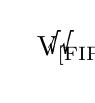
\begin{tikzpicture}[baseline=(root.base), sibling distance=0.7cm]
    \Tree
    [.\node(root){V\makebox[0pt][l]{\textsubscript{[FIP:\uline{V}]}}}; [.{Cat\makebox[0pt][l]{\textsubscript{[FIP:\uline{\hspace{3mm}}]}}} {Cat\makebox[0pt][l]{\textsubscript{[FIP:\uline{\hspace{3mm}}]}}} {\textsurd1} ] [.{V\makebox[0pt][l]{\textsubscript{[FIP:\uline{V}]}}} {\emph{v}\makebox[0pt][l]{\textsubscript{[FIP:\uline{V}]}}} {\textsurd2} ] ]
\end{tikzpicture}\vskip\medskipamount
\ex 
\begin{tikzpicture}[baseline=(root.base), sibling distance=0.7cm]
    \Tree
    [.\node(root){V\makebox[0pt][l]{\textsubscript{[FIP:\uline{V}]}}}; [.{Cat\makebox[0pt][l]{\textsubscript{[FIP:\uline{\hspace{3mm}}]}}} {Cat\makebox[0pt][l]{\textsubscript{[FIP:\uline{\hspace{3mm}}]}}} {$\sqrt{\textrm{\textsc{hand}}}$} ] [.{V\makebox[0pt][l]{\textsubscript{[FIP:\uline{V}]}}} {\emph{v}\makebox[0pt][l]{\textsubscript{[FIP:\uline{V}]}}} {$\sqrt{\textrm{\textsc{wash}}}$} ] ]
\end{tikzpicture}
\z
\z

\noindent Suppose the system can distinguish intrinsically valued features from
features valued via \isi{Agree},\footnote{I leave aside the technical details, but any
adequate theory would be compatible. See \citet[10]{RooryckWyngaerd2011} for a
proposal based on feature sharing.} there would be a derivational asymmetry
between Cat\textsubscript{\textsurd} and V\textsubscript{\textsurd}, with the
former's interpretation depending on the latter's. This dependency may be
reflected in semantics as variable sharing, which I briefly illustrate below.

Under the bare Root view, I assume that the denotation of a Root is radically
underspecified, to the extent that it is not only grammatically void, but also
does not make a complete function. Instead, a Root merely denotes a vague
property -- a ``function template'' whose domain (including variable type) is
not yet defined, as in \REF{ex:sema}. This information is only added when the
Root is categorized, as in \REF{ex:semb}.

\ea\label{ex:sem}
\ea\label{ex:sema}
{\upshape
$⟦\sqrt{\textrm{\textsc{wash}}}⟧$ = $\lambda$\uline{\hspace{3mm}} .\textsc{wash}({\uline{\hspace{3mm}}})\\ =  `encyclopedically related to wash and compositionally \uline{\hspace{3mm}}'}
\ex\label{ex:semb}
{\upshape
$⟦$[{\em v} $\sqrt{\textrm{\textsc{wash}}}$]$⟧$ = $\lambda e$.\textsc{wash}($e$)\\ = `encyclopedically related to wash and compositionally an extending-into-time \gls{FIP} (i.e.\ an event)'
}
\z
\z

\largerpage[-1]
The event variable $e$ in \REF{ex:semb}, which defines eventuality, is
introduced by the verbalizer \citep[cf.][]{Marantz2013}. Since the verbalizer
is featurally [FIP:V], $e$ is presumably encoded in the value [V]. More
generally, I assume all variable types to be functionally introduced rather
than an inherent part of the Root. Being valueless, Cat does not introduce any
variable type, though it does endow the Root with interface interpretability
(as an FIP).\footnote{A consequence of the single engine hypothesis is that
    unvalued features must not be deleted by the end of the categorizer phase\is{phases}
    (i.e.\ when the categorized Roots are renumerated), because they are still
    required in the Chomskyan numeration and the next cycle of derivation. I
    merely acknowledge this point but do not attempt to account for it in this
study.} So, Cat\textsubscript{\textsurd} has the denotation in \REF{ex:sem2}.

\ea\label{ex:sem2}
\ea\label{ex:sem2a}
{\upshape
$⟦$[Cat {\textsurd1}]$⟧$ =
$\lambda$$⟦$[FIP:\uline{\hspace{3mm}}]$⟧$.1($⟦$[FIP:\uline{\hspace{3mm}}]$⟧$)\\
= `encyclopedically related to 1 and compositionally a \uline{\hspace{3mm}}
FIP'
}
\ex\label{ex:sem2b}
{\upshape
$⟦$[Cat $\sqrt{\textrm{\textsc{hand}}}$]$⟧$ =
$\lambda$$⟦$[FIP:\uline{\hspace{3mm}}]$⟧$.\textsc{hand}($⟦$[FIP:\uline{\hspace{3mm}}]$⟧$)\\
= `encyclopedically related to hand and compositionally a
\uline{\hspace{3mm}} \gls{FIP}'

}
\z
\z

\noindent After \isi{Agree}, Cat\textsubscript{\textsurd} is equipped with the event variable introduced by {\em v}. However, since the categorial interpretation of {\textsurd1} has been fixed in the previous spell-out cycle, the newly obtained $e$ can no longer turn {\textsurd1} into an independent event, but only connects it to another event, i.e.\ that denoted by V\textsubscript{\textsurd}. As such, {\textsurd1} effectively becomes a modifier of V\textsubscript{\textsurd}, as in \REF{ex:sem3}.

\ea\label{ex:sem3}
\ea\label{ex:sem3a}
{\upshape
$⟦$(\ref{ex:catx}a)$⟧$ = $\lambda \uline{e}$.1($\uline{e}$) $\wedge$ $\lambda e$ .2($e$)\\ = `encyclopedically related to 1 and compositionally connected to an event' $\wedge$ `encyclopedically related to 2 and compositionally an event' \\ = `an event of 2, encyclopedically related to 1' \hfill (event identification)
}
\ex\label{ex:sem3b}
{\upshape
$⟦$(\ref{ex:catx}b)$⟧$ = $\lambda \uline{e}$.\textsc{hand}($\uline{e}$) $\wedge$ $\lambda e$ .\textsc{wash}($e$)\\ = `encyclopedically related to hand and compositionally connected to an event' $\wedge$ `encyclopedically related to wash and compositionally an event' = `an event of washing, encyclopedically related to hand'
}
\z
\z

Since \{Cat\textsubscript{\textsurd}, V\textsubscript{\textsurd}\} and
V\textsubscript{\textsurd} have identical labels, Cat\textsubscript{\textsurd}
is in effect an adjunct. Since Cat\textsubscript{\textsurd} is dominated by V,
it is verb-internal. The modificational compound\is{compounding} is thus derived solely by Simplest \isi{Merge} and labeling\is{labelling}, with no need of Pair \isi{Merge}, Root \isi{incorporation}, postsyntactic operation or \isi{multidominance}. In effect, the structure in \REF{ex:catx} unifies two Roots under one ordinary categorizer without violating the \gls{DM} tenet that one categorizer can only categorize one Root \citep[cf.][]{Embick2010}.

\section{Some implications}\label{sec5}

\subsection{Noun-internal modifiers}\label{sec5.1}

In \Cref{sec4}, I illustrated how \glspl{VIM}\is{verb-internal modifiers} are derived by Cat, but the
application of the defective categorizer hypothesis is not confined to the
verbal domain. In fact, since all Cat\textsubscript{\textsurd} needs is an
\gls{FIP} value, it may well be merged with a noun and become a \gls{NIM}.
While leaving \glspl{NIM} to future research, in \REF{ex:nim} I illustrate the
flexibility of Cat by items that can be used as both \gls{VIM} and NIM.

\ea\label{ex:nim}
\ea {English}\\
hand{\textsubscript{[FIP:\uline{V}]}}-wash{\textsubscript{[FIP:V]} vs.} hand{\textsubscript{[FIP:\uline{N}]}}-gel{\textsubscript{[FIP:N]},}\\
sleep {\textsubscript{[FIP:\uline{V}]}}-walk{\textsubscript{[FIP:V]} vs.} sleep{\textsubscript{[FIP:\uline{N}]}}-mode{\textsubscript{[FIP:N]},}\\
breast{\textsubscript{[FIP:\uline{V}]}}-feed{\textsubscript{[FIP:V]} vs.} breast{\textsubscript{[FIP:\uline{N}]}}-bone{\textsubscript{[FIP:N]}%\dots
}
\ex {Chinese}\\
sh\v{o}u{\textsubscript{[FIP:\uline{V}]}}-x\v{\i}{\textsubscript{[FIP:V]} `hand-wash; to handwash'} {vs.}\\
sh\v{o}u{\textsubscript{[FIP:\uline{N}]}}-j\={\i}{\textsubscript{[FIP:N]} `hand-machine; mobile phone',}\\
x\={\i}n{\textsubscript{[FIP:\uline{V}]}}-su\`{a}n{\textsubscript{[FIP:V]} `heart-calculate; to do mental calculation'} {vs.}\\
x\={\i}n{\textsubscript{[FIP:\uline{N}]}}-l\`{\i}{\textsubscript{[FIP:N]} `heart-force; mental efforts'}\\
%d\`{a}{\textsubscript{[FIP:\uline{V}]}}-xi\`{a}o{\textsubscript{[FIP:V]} `big-laugh; to laugh loudly'} {vs.}\\
%d\`{a}{\textsubscript{[FIP:\uline{N}]}}-r\'{e}n{\textsubscript{[FIP:N]} `big-person; adult'\dots
%}
\ex {Japanese}\\
se{\textsubscript{[FIP:\uline{V}]}}-ou{\textsubscript{[FIP:V]} `back-carry; to carry on back'} {vs.}\\
se{\textsubscript{[FIP:\uline{N}]}}-bone{\textsubscript{[FIP:N]}} {`back-bone',}\\
oshi{\textsubscript{[FIP:\uline{V}]}}-taosu{\textsubscript{[FIP:V]} `push-topple; to push down'} {vs.}\\
oshi{\textsubscript{[FIP:\uline{N}]}}-bana{\textsubscript{[FIP:N]}} {`push-flower; pressed flower'}\\
%chika{\textsubscript{[FIP:\uline{V}]}}-zuku{\textsubscript{[FIP:V]} `close-attach; to get near'} {vs.}\\
%chika{\textsubscript{[FIP:\uline{N}]}}-michi{\textsubscript{[FIP:N]}} {`close-way; shortcut'\dots
%}
\z
\z

The Cat-licensed Roots $\sqrt{\textrm{\textsc{hand}}}$,
$\sqrt{\textrm{\textsc{sleep}}}$, $\sqrt{\textrm{\textsc{breast}}}$, etc.\ have
no fixed \gls{FIP} interpretation -- they become \glspl{VIM}\is{verb-internal
modifiers} when merging with V\textsubscript{\textsurd}s and NIM when
merging with N\textsubscript{\textsurd}s. Admittedly, whether or not a specific
Cat-item has both verbal and nominal uses is a matter of language-specific
lexicalization, e.g.\ while all of {\it hand-wash}, {\it hand-gel}, and {\it
foot-gel} are fine in \ili{English}, there is no ?{\it foot-wash} (`wash with
foot') by the time this chapter is written (though it could easily be coined).
The defective categorizer hypothesis does not aim to predict which
\glspl{VIM}/NIMs actually exist in a certain language, but merely
captures the capacity of human beings to create such language units.

\subsection{Universality of compounding}\label{sec5.2}

The proposed theory can not only be extended to the nominal domain but also
predict the widespreadness of modificational compounds. Given the mutual
dependence between feature classes (attributes) and features (values), the
\gls{FIP} class (i.e.\ the set of \gls{FIP} values) should be as widespread as
its values. Moreover, if ``no value'' can be conceived as the empty set, i.e.
[F:\uline{\hspace{3mm}}]\,=\,[F:$\varnothing$], then unvalued features are in
effect free-riders of their valued counterparts, for the empty set is a subset
member of all sets, which include all feature classes (conceived as subsets of
all features, cf.\ \Cref{sec3.2}). This means any language with at least one
\gls{FIP} value also has a grammatically active defective categorizer. In other
words, modificational \isi{compounding} as a generative mechanism is as widespread in
human languages as conventional \isi{lexical categories}, i.e.\ universal (cf.\
\citealt{Baker2003,Panagiotidis2015}).

This conclusion is supported by typological studies. According to
\citet[344]{Bauer2009}, (modificational) \isi{compounding} has been suggested to be a
language universal (\citealt[54--55]{FromkinEtal1996};
\citealt[2]{Libben2006}), as evidenced by language acquisition\is{language acquisition}
\citep{Clark1993} and contact \citep{Plag2006}. A caveat here is that
universality may be masked by varied terminology and classification in
descriptive grammars. For example, descriptions of Ainu (e.g.\
\citealt{Refsing1986,Shibatani1990}) do not mention \isi{compounding} at
all, though the language does have de facto compounds, as in
\REF{ex:ainu}.  Similarly, \ili{Evenki} has also been claimed to lack compounds
\citep[308]{Nedjalkov1997}, but a quick look into alternative sources reveals
many of them, as in \REF{ex:evenki}.

\ea
\ea\label{ex:ainu}\il{Ainu}
\langinfo{Ainu}{language isolate}{\citealt[via][]{Bauer2009}}\\
atuy asam {`bottom sea; sea bottom',} kamuy napuri {`mountain god; holy mountain',} supuya kur {`trace smoke; smoke trace'}
\ex\label{ex:evenki}\il{Evenki}
\langinfo{Evenki}{Tungusic}{\citealt[cf.][]{HuChao1986}}\\
eyji shee {`brick tea',} aaxin jolo {`liver stone; marble',} unaaji ute {`girl son; daughter'}
\z
\z

\subsection{Compound verb typology}\label{sec5.3}

Despite the universality of modificational compounds, compound nouns are\linebreak
cross-linguistically a lot more common than compound verbs. Take the familiar
Eu\-ro\-pean languages for example: while modificational compound nouns exist
in all of \ili{Germanic}, \ili{Romance}, and \ili{Slavic} languages \citep[cf.][]{Bauer2009},
compound verbs like {\it hand-wash} are only seen in \ili{English} with some
productivity. One might take this to be an areal phenomenon, for compound verbs
are more widely used in e.g.\ East Asia. However, as \citet[355]{Bauer2009}
comments, the areal preferences are not clearly correlated ``with anything
linguistic in the appropriate languages''.

The defective categorizer hypothesis provides a new perspective on modeling
this unbalanced typology. Since the node dominating
[Cat\textsubscript{\textsurd} V\textsubscript{\textsurd}] (call it
$\mathbb{V}$\footnote{Similar to \posscitet{Booij1990} V*, which is more than
V\textsuperscript{0} but less than Vʹ \citep[cf.][]{Vikner2005}.}) has exactly
the same label as the V\textsubscript{\textsurd} node, operations targeting one
node also target the other. As a result, in languages requiring V-to-T/C
movement, the T/C probe is unable to access the real V\textsuperscript{0} (i.e.
V\textsubscript{\textsurd}, which becomes a terminal lexical item after
renumeration, cf.\ \Cref{sec4.3}) due to the intervening $\mathbb{V}$, as in
\REF{ex:move}. This is presumably a minimal search effect, as formulated in the
minimal link condition \REF{ex:mlc}.

\ea\label{ex:move}
    
\begin{tikzpicture}[baseline=(root.base), sibling distance=0.7cm]%, scale=0.9]

        \Tree   [.\node(root){\dots};
                    \node(tc){T/C\makebox[0pt][l]{\textsubscript{=Probe}}};
                    [.{\dots}
                        {\dots}
                        [.\node(v+){$\mathbb{V}$\makebox[0pt][l]%
                            {\textsubscript{=Goal}}};
                            {Cat\makebox[0pt][l]{\textsubscript{\textsurd}}}
                            \node(v){V\makebox[0pt][l]%
                                {\textsubscript{\textsurd=Goal}}};
                        ]
                    ]
                ]

        \draw [->, bend left=50] (v.south west) to
            node[pos=.5, below]{\ding{55}}(tc.south);
        \draw [->, bend left=50] (v+.south west) to
           node[pos=.5, below]{\ding{55}}(tc.south);

%        \draw[semithick, ->] (v)..controls +(south west:1) and
%            +(south:3)..(tc)node[pos=0.5,above]{\ding{55}};
%
%        \draw[semithick, ->] (v+)..controls +(south west:1) and +(south
%            east:3)..(tc)node[pos=0.5,above]{\ding{55}};

    \end{tikzpicture}
\ex \label{ex:mlc} Minimal link condition \citep[311]{Chomsky1995}:\\
    K attracts {α} only if there is no {β}, {β} closer to K than {α}, such that
    K attracts β.
\z

In addition, since $\mathbb{V}$ is not a minimal category (head) on the clausal
spine, it cannot undergo \isi{head movement} either (see \ref{ex:move}).
Therefore, in the end nothing moves to T/C, and the derivation crashes. This
means Cat--V compound verbs are only well-formed in languages/contexts without
verb movement requirement. So \ili{Romance} languages, where V systematically moves
to T \citep[cf.][]{BiberauerRoberts2010}, are incompatible with such compound
verbs.  For instance, the concepts in \REF{ex:mod} are expressed
periphrastically in \ili{Spanish}, as in \REF{ex:spa}.\footnote{Retrieved from
oxforddictionaries.com and wordreference.com (29 Dec 2017).}

\ea\label{ex:spa}
{\upshape
\begin{tabular}[t]{ll}
English & Spanish\\
{\it double-check} & {\it volver a revisar} `to inspect again'\\
%{\it second-guess} & {\it cuestionar a posteriori} `to question in hindsight'\\
%{\it proof-read} & {\it corregir} `to correct' \\
{\it dry-clean} & {\it limpiar en seco} `to clean in dry' \\
{\it hand-wash} & {\it lavar a mano} `to wash by hand'\\
%{\it stir-fry} & {\it saltear} `to saut\'{e}'\\
{\it sleep-walk} & {\it caminar dormido} `to walk asleep' \\
{\it window-shop} & {\it mirar escaparates} `to look at shop windows'\\
{\it baby-sit} & {\it hacer de canguro} `to do kangaroo'\\
%{\it breast-feed} & {\it amamantar} `to breastfeed'\\
{\it hitch-hike} & {\it hacer autoestop} `to do car-stop'\dots \\
\end{tabular}}
\z

However, the prediction as such is too strong, for apart from V-to-T/C, there
is also V-to-{\em v}* (or more generally V-to-VP-shell) movement, e.g.\ in
\ili{English} (cf.\ Roberts \citeyear{Roberts2010}, \citeyear{Roberts2019}).
So, if Cat--V compounds and \isi{verb movement} are totally complementary, then
\ili{English} becomes a major counterexample.

One possible solution lies in the design of Cat. Since it merely needs to merge with something that can provide it with an \gls{FIP} value (and thus label the merger), which in the case of [V] is essentially an event variable, it can in theory merge with any $e$-equipped head. In a neo-constructionist event structure \citep[cf.][]{Acedo2016}, this may be any subevental head (e.g.\ Init/Proc/Res in \citealt{Ramchand2008}) or argument introducing head (e.g.\ Voice/Appl in \citealt{Pylkkanen2008}). Considering Internal \isi{Merge} occurs at phase\is{phases} level \citep[cf.][]{Citko2014}, i.e.\ after all steps of External \isi{Merge} in a phase\is{phases} are done, and the Cat\textsubscript{\textsurd}-V\textsubscript{\textsurd} merger is External \isi{Merge}, here I make the conservative hypothesis that apart from the verbalizer, the next position Cat may attach to is the {\em v}* phase\is{phases} head (whichever head that turns out to be in an elaborate verbal domain). Crucially, since Cat only merges in after all steps of Internal \isi{Merge} in {\em v}*P are done (i.e.\ as part of the next phase\is{phases}), Cat--V (more exactly Cat-{\em v}*) compounds may well exist in a language with V-to-{\em v}* movement. In sum, we can have a three-way typology of Cat--V compounds (and \glspl{VIM}) regulated by the \isi{verb movement} parameter, as in \tabref{tab:typology}.

\begin{table}
\caption{Typology of Cat--V compound verbs}
\label{tab:typology}
 \begin{tabular}{clcc}
  \lsptoprule
   Type &Example & V-to-T/C movement & Cat--V compound\\
  \midrule
  I  &  \ili{Romance}  & Yes  & No \\
  II  & OV-Germanic & Main clause: Yes &  No\\
  II  & OV-Germanic & Embedded clause: No & Yes\\
 III & \ili{English}, Chinese & No & Yes\\
  \lspbottomrule
 \end{tabular}
\end{table}\il{English}\il{Romance}

\noindent Note that due to the inconsistent \isi{verb movement} requirement, OV-Germanic languages may only have Cat--V compounds in non-V2 contexts, as in \REF{ex:immobile}.\largerpage

\ea\label{ex:immobile}
\langinfo{German}{}{\citealt[via][]{Vikner2005}}\\
\ea[*]{
\gll Spart er bau? {/ *} Bau-spart er? \\
     saves he building {} building-saves he\\
\glt (`Does he building-save?')}
\ex[]{
    \gll Er will bau-sparen. / \dots{} weil er bau-spart.\\
    he wants building-save.\Inf{} {} {} because he building-saves\\
\glt `He wants to building-save.\slash\dots because he building-saves.'
}
\z
\z

\noindent The compound verb {\it bau-sparen} `building-save; to building-save'
cannot appear in finite main clauses but is only well-formed in situ, either
in a sentence with a modal verb (which fulfills the V2 requirement) or in a
subordinate clause (where there is no V2 requirement). \ili{Germanic} compounds like
{\it bau-sparen} are known as ``immobile verbs'' (cf.\ i.a.\
\citealt{Mcintyre2002,Vikner2005,Ahlers2010,Song2016}). They have a
natural explanation in the current model.

As a final remark, the typology in \tabref{tab:typology} only concerns Cat--V
compounds. So, on the one hand, Type I--II languages may still have unhindered
Cat-N compounds/NIMs, e.g.\ French {\it homme grenouille} `man-frog;
frogman', \ili{Spanish} {\it boca-calle} `mouth-street; street intersection'. On the
other hand, they may also have other types of complex verb in all contexts,
such as particle verbs (including their inseparable variants), e.g.\ \ili{German}
{\it ein-kaufen} `in-buy; to shop' (V-PP), {\it er-warten} `{\sc er}-wait; to
expect' ({\it er}<OHG {\it ur} `out'), \ili{Spanish} {\it ex-traer} `out-pull; to
extract', and various phrasal verbs, e.g.\ French {\it mettre bas} `put low; to
give birth' (V+AP), \ili{Spanish} {\it ponerse en camino} `put.{\sc refl} on way; to
set off' (V+clitic+PP), \ili{German} {\it Schwein haben} `pig have; to be lucky'
(V+NP). I do not discuss these other types of complex verb (more exactly
complex predicate) but merely distinguish them from Cat--V compounds. To wit,
items like {\it ein}, {\it bas}, and {\it Schwein} are base-generated as
V-complements, i.e.\ \glspl{VM} in the broad sense (cf.\ \Cref{sec1}), but they
are not \glspl{VIM}\is{verb-internal modifiers}.

\section{Conclusion}\label{sec6}

This chapter is a minimalist study of verb-internal modifiers (non-heads of
modificational compound verbs). I have defended the position that compounding
is a syntactic phenomenon based on the view that syntax is the only generative
engine in the human language faculty. My main difference from previous
syntactic models of \isi{compounding} is that I have kept to the simplest definition
of \isi{Merge} (no Pair \isi{Merge} or remerge) and the bare Root view (no RootP, Root-Root
merger or Root \isi{incorporation}), both of which are consequences of the \gls{SMT}.
Guided by the defective categorizer hypothesis, which is independently
motivated in the minimalist feature system, I have derived \glspl{VIM}\is{verb-internal modifiers} in a
labeling-based model. This new model not only avoids the conceptual problems in
previous approaches, but also brings along a number of potential points of
future research. First, it can be extended to the nominal domain and allows the
same Root material to modify both verbs and nouns. Second, it predicts
modificational \isi{compounding} to be a language universal and relates the typology
of Cat--V compounds to the \isi{verb movement} parameter. In addition, beyond the
verbalizer level, there may be further loci that Cat can attach to, e.g.\ the
{\em v}* phase\is{phases} head. As such, \isi{compounding} is not only a natural part of syntax,
but also sheds new light on ``external'' syntactic issues such as general head
adjunction and phase-level modifiers.



\printchapterglossary{}

\section*{Acknowledgements}

This study forms part of my PhD project ``Flexibility of syntactic categories: A
cross-linguistic study'' (funded by Cambridge Trust and China Scholarship
Council). I am grateful to Ian Roberts, Theresa Biberauer, Anders Holmberg and
V\'{\i}ctor Acedo-Matell\'{a}n for discussions and encouragement. Thanks to the
anonymous reviewer for helpful feedback, and to the audience at the Cambridge
SyntaxLab (2 February 2016, 7 February 2017), the ``Linguistic variation in the
interaction between internal and external syntax'' workshop (Utrecht, 8--9 Feb
2016), and the graduate conference WoSSP13 (Barcelona, 30 June--1 July 2016)
for questions and comments on earlier versions of this work. All remaining
errors are my own.

{\sloppy\printbibliography[heading=subbibliography,notkeyword=this]}

\end{document}
